%% Road to VPhO 2023 Template

\documentclass[12pt]{article}
\usepackage[english]{babel}
\usepackage[T5]{fontenc}
\usepackage[top=2cm, bottom=2cm, left=2cm,right=2cm]{geometry} %%%% Margin %%%%%
\usepackage[dvipsnames]{xcolor}
\usepackage[pdftex]{graphicx}
\usepackage{wrapfig}
\usepackage{tcolorbox}
\usepackage{mathtools}
\usepackage{amsmath}
\usepackage{amssymb}
\usepackage{eqnarray}
\usepackage{siunitx}
\usepackage{array, lipsum, bibentry,fancyhdr}
\usepackage{hyperref}
\usepackage{natbib}
\setlength{\parindent}{0pt}
\usepackage{enumitem}
\usepackage[noframe]{showframe}
\usepackage{framed}
\usepackage{titling}
\usepackage{float}
\usepackage{multicol}
\usepackage{url}
\usepackage{authblk}
\usepackage{sectsty}
\usepackage{eqparbox}

%%%%%%%%%% Pictures drawing %%%%%%%%%%%%%

\usepackage{pgfplots} %%%%%% Regression %%%%
\pgfplotsset{compat = newest}
\usepackage{pgfplotstable}
\usepackage{tikz}
\usepackage{tikz-3dplot} %%%%%% Draw %%%%%%
\usepackage{tikz,tkz-euclide}
\usetikzlibrary{arrows,calc,patterns}
\usetikzlibrary{quotes,angles}
\usetikzlibrary{shapes.geometric}
\usepackage{circuitikz} %%%%% Circuit %%%%
\usetikzlibrary{decorations.pathmorphing,patterns}

\setlength{\unitlength}{1cm}

%%%%%%%%%% Hyperlink %%%%%%%%%%%%%

\hypersetup{
	colorlinks=true,
	linkcolor=black,
	filecolor=mangeta,      
	urlcolor=blue,
	pdftitle={Overleaf Example},
	pdfpagemode=FullScreen,
}

%%%%%%%%%% Header & Footer %%%%%%%%%%%%%

\setlength{\headheight}{10mm}
\RequirePackage{fancyhdr}  % Needed to define custom headers/footers
\RequirePackage{lastpage}  % Number of pages in the document
\pagestyle{fancy}          % Enables the custom headers/footers
% Headers
\lhead{\includegraphics[width=.8in]{xPhO.png}}%
\chead{}%
\rhead{\small\sffamily\bfseries{Đề bài hướng tới VPhO 42} --- \thepage/\pageref{LastPage}}
% Footers
\lfoot{}%
\cfoot{}%
\rfoot{}%
\renewcommand{\headrulewidth}{1pt}% % header rule
\renewcommand{\footrulewidth}{1pt}% % footer rule

% \pagestyle{fancy}
% 	\fancyhead[L]{\empty}
% 	\fancyhead[R]{\empty}
% 	\fancyhead[C]{\empty}
% 	\fancyfoot[C]{\empty}
% 	\fancyfoot[L]{\empty}
% 	\renewcommand{\headrulewidth}{0pt}
% 	\fancyfoot[C]{\normalcolor{\thepage/\pageref{LastPage}}}
% 	\setcounter{page}{1}

%%%%%%%%%% Color setup %%%%%%%%%%%%%

\RequirePackage{xcolor}
\definecolor{wsdred}{HTML}{8E1728}
\definecolor{wsdgrey}{HTML}{75787B}
\renewcommand{\normalcolor}{\color{wsdred}}
\colorlet{ColorOr}{white}

\begin{document}

%% Title %%
{\fontsize{50}{24}\fontfamily{phv}\fontseries{b}
\LARGE \normalcolor{Đề bài hướng tới VPhO 42} }

\textcolor{blue}{\textbf{\textit{Câu lạc bộ vật lý xPhO}}}

%%%%
\vspace{5mm}

{\normalcolor\textbf{CÂU 1. (4.0 điểm)}}\vspace{1.5mm}

\setcounter{equation}{0}
%Bổ sung lệnh vẽ lò xo
\usetikzlibrary{patterns,snakes}
\tikzstyle{spring}=[line width=0.8,blue!7!black!80,snake=coil,segment amplitude=5,segment length=5,line cap=round]

\textbf{Khối lượng âm...}

% Vào đầu thế kỷ XXI, một số nghiên cứu mới về một loại vật liệu nhân tạo được tạo bởi các cấu trúc tuần hoàn như những mạng tinh thể được gọi là \textit{metamaterial} đã mang tới một số tính chất kỳ lạ mà vật liệu tự nhiên không thể có được. Trong đó, ở lĩnh vực cơ học, loại siêu vật liệu này cho phép ta thu được "khối lượng hiệu dụng âm", "hệ số Poisson âm", "suất Young âm",... tạo ra nhiều tiềm năng ứng dụng cho các phòng cách âm hoàn hảo, siêu thấu kính,... Trong bài toán này, ta sẽ khảo sát mô hình "khối lượng trong khối lượng" (mass-in-mass model) và hiện tượng khối lượng âm của loại vật liệu này.
Ở thế giới bình thường của chúng ta, khối lượng âm là điều không tưởng. Trong một số mô hình truyền sóng cơ học, khối lượng hiệu dụng của các thành phần trong mạng tinh thể nhân tạo có thể âm và đưa đến những tính chất thú vị. Một trong những mô hình đơn giản hóa và tiêu biểu của khối lượng hiệu dụng âm là mô hình "khối lượng trong khối lượng" (mass-in-mass model).

\begin{enumerate}
\item \textbf{Mô hình mạng nguyên tử tinh thể và sóng đàn hồi.} \\
Xét một mạng tinh thể một chiều gồm các hạt khối lượng $m$ đặt cách đều nhau một khoảng $L$ như hình \ref{fig1_negative_mass}. Xem như mỗi hạt "nguyên tử" trong mạng chỉ tương tác với hai hạt liền kề nó và tương tác này tương đương với một lò xo độ cứng $k$, độ dài tự nhiên $L$. Với hạt thứ $n$ trong mạng tinh thể, vị trí cân bằng của hạt này là tại $x_n=nL$. Ta ký hiệu li độ của hạt thứ $n$ này so với vị trí cân bằng là $u_n$.

\begin{center}
\begin{tikzpicture}
    \draw[spring] (0.3,0)--++(1.4,0);
    \draw[spring] (2.3,0)--++(1.4,0);
    \draw[spring] (4.3,0)--++(1.4,0);
    \draw[spring] (6.3,0)--++(1.4,0);
    \draw[spring] (8.3,0)--++(1.4,0);
    \draw[spring] (10.3,0)--++(1.4,0);
    \draw[dashed] (-0.3,0)--(0.3,0) (11.7,0)--(12.3,0);
    \filldraw[color=black, fill=gray, ultra thick](2,0) circle (0.3);
    \filldraw[color=black, fill=gray, ultra thick](4,0) circle (0.3);
    \filldraw[color=black, fill=gray, ultra thick](6,0) circle (0.3);
    \filldraw[color=black, fill=gray, ultra thick](8,0) circle (0.3);
    \filldraw[color=black, fill=gray, ultra thick](10,0) circle (0.3);
    % \draw (2,0.5) node[above]{$n-2$} (4,0.5) node[above]{$n-1$} (6,0.5) node[above]{$n$} (8,0.5) node[above]{$n+1$} (10,0.5) node[above]{$n+2$};
    \draw (2,-1) node[below]{$(n-2)L$} (4,-1) node[below]{$(n-1)L$} (6,-1) node[below]{$nL$} (8,-1) node[below]{$(n+1)L$} (10,-1) node[below]{$(n+2)L$};
    \draw[-Stealth] (-1,-1)--(13,-1);
    \draw (2,-1.1)--(2,-0.9) (4,-1.1)--(4,-0.9) (6,-1.1)--(6,-0.9) (8,-1.1)--(8,-0.9) (10,-1.1)--(10,-0.9);
    \filldraw[color=black, fill=black, ultra thick](-0.5,-1) circle (0.05);
    \draw (-0.5,-0.9) node[above]{$O$} (12.5,-0.9) node[above]{$x$};
    \draw (2,0.8)--(2,1.2) (4,0.8)--(4,1.2) (6,0.8)--(6,1.2) (8,0.8)--(8,1.2) (10,0.8)--(10,1.2);
    \draw[->] (2,1)--(2.7,1);
    \draw[->] (4,1)--(4.7,1);
    \draw[->] (6,1)--(6.7,1);
    \draw[->] (8,1)--(8.7,1);
    \draw[->] (10,1)--(10.7,1);
    \draw (2.4,1) node[above]{$u_{n-2}$} (4.4,1) node[above]{$u_{n-1}$} (6.4,1) node[above]{$u_n$} (8.4,1) node[above]{$u_{n+1}$} (10.4,1) node[above]{$u_{n+2}$};
\end{tikzpicture} \\
\vspace{3mm}
Hình 1: Mô hình mạng tinh thể.
\label{fig1_negative_mass}
\end{center}

    \begin{enumerate}[label=\textbf{\alph*,}]\itemsep0em
        \item Chứng minh rằng, li độ và gia tốc của các hạt trong mạng tinh thể tuân theo phương trình sai phân sau:
        $$ \ddot{u}_n = -\dfrac{k}{m} \left( 2 u_n - u_{n+1} - u_{n-1} \right).$$
        \item Với một sóng kích thích có tần số cương bức $\omega$ tác động lên mạng tinh thể, chọn gốc tọa độ $n=0$ và gốc thời gian $t=0$ phù hợp, ta có thể tìm nghiệm của hệ phương trình sai phân trên có thể được tìm dưới dạng
        $$ u_n = A \sin \left( \dfrac{\omega}{v} x_n \right) \cos ( \omega t ),$$
        trong đó $A$ là biên độ và là một hằng số, $v$ là vận tốc truyền sóng trong mạng tinh thể. Tìm vận tốc truyền sóng $v$ theo $\omega$, $m$, $k$ và $L$ trong mô hình này.
        \item Chỉ ra rằng: Với $L$ vô cùng bé so với các đại lượng khác cùng thứ nguyên, môi trường truyền sóng gần như liên tục, vận tốc truyền sóng sẽ không phụ thuộc vào $\omega$. Xem rằng trung bình mỗi mạng tinh thể dọc trong vật liệu được mô tả như trên nằm trong một vùng diện tích $\Delta S$ trên mặt cắt ngang. Tìm vận tốc truyền sóng này theo khối lượng riêng $\rho$ và suất Young $E$ của vật liệu.
    \end{enumerate}
\item \textbf{Mô hình "khối lượng trong khối lượng" và hiện tượng "khối lượng âm"} \\
Để cải tiến mô hình mạng tinh thể và thu được những tính chất thú vị, ta thay thế "hạt nguyên tử" trên thành một hạt kiểu mới, gồm một hạt khối lượng $m_1$ nối với một hạt $m_2$ (với $m_2<m_1$) bằng một lò xo có độ cứng $k_2$ như hình \ref{fig2_negative_mass}. 

\begin{center}
\begin{minipage}{0.4\textwidth}
\centering
\begin{tikzpicture}
    \filldraw[color=black, fill=gray, ultra thick](0,0) circle (1.5);
    \filldraw[color=black, fill=white, ultra thick](0,0) circle (1.3);
    \draw[spring] (-1.3,0)--++(1.8,0);
    \filldraw[color=black, fill=gray, ultra thick](0.7,0) circle (0.2);
    \draw (-0.3,0.2) node[above]{$k_2$} (0.7,0.2) node[above]{$m_2$} (-1.3,1.2) node[above]{$m_1$};
    \draw[thick,-Stealth] (-2,-2.5)--(2,-2.5);
    \draw (0,-2.5) node[above]{$F=F_0 \cos (\omega t)$};
\end{tikzpicture}
\end{minipage}
% \hspace{0.1\textwidth}
\begin{minipage}{0.4\textwidth}
\centering
\begin{tikzpicture}
    \filldraw[color=black, fill=gray, ultra thick](0,0) circle (1.5);
    % \filldraw[color=black, fill=white, ultra thick](0,0) circle (1.3);
    % \draw[spring] (-1.3,0)--++(1.8,0);
    % \filldraw[color=black, fill=gray, ultra thick](0.7,0) circle (0.2);
    % \draw (-0.3,0.2) node[above]{$k_2$} (0.7,0.2) node[above]{$m_2$} (-1.3,1.2) node[above]{$m_1$};
    \draw (-1.3,1.2) node[above]{$m_{eff}$};
    \draw[thick,-Stealth] (-2,-2.5)--(2,-2.5);
    \draw (0,-2.5) node[above]{$F=F_0 \cos (\omega t)$};
\end{tikzpicture}
\end{minipage}
\\
\vspace{5mm}
Hình 2: Một cơ hệ (hình bên trái) được tương đương như một hạt "nguyên tử" mới trong mạng tinh thể (hình bên phải).
\label{fig2_negative_mass}
\end{center}

Khảo sát độc lập một hạt mới này, ta xem lực mà các hạt khác xung quanh tác dụng lên hạt khối lượng $m_1$ như một lực cưỡng bức điều hòa $F$ với tần số cưỡng bức $\omega$. Do chịu ảnh hưởng bởi lực tác động trên, hạt $m_1$ bị cưỡng bức và dao động dưới tần số $\omega$, li độ của $m_1$ khi đó có thể viết dưới dạng
$$u = -\dfrac{F}{m_{eff} \omega^2}.$$
Với $m_{eff}$ được gọi là khối lượng hiệu dụng của cơ hệ.
Xác định khối lượng hiệu dụng của hạt mới $m_{eff}$ theo $m_1$, $m_2$, $k_2$ và $\omega$.
Với những giá trị nào của tần số $\omega$ thì khối lượng hiệu dụng $m_{eff}$ âm? 

    % \begin{enumerate}[label=\textbf{\alph*,}]\itemsep0em
    %     \item Xác định khối lượng hiệu dụng của hạt mới $m_{eff}$ theo $m_1$, $m_2$, $\omega_0$ và $\omega$.
    %     \item Vẽ phác đồ thị $m_{eff}$ theo tần số kích thích $\omega$. Với những giá trị nào của tần số $\omega$ thì khối lượng hiệu dụng âm? 
    % \end{enumerate}
\end{enumerate}

\textit{Ghi chú: Trong bài toán này, ta xem như các lực ma sát và các tổn thất năng lượng là rất nhỏ để đưa vào tính toán, song nó vẫn tồn tại để các dao động tự do nhanh chóng bị tắt.}

\begin{flushright}
    (Biên soạn bởi Log và $\tau \hbar \alpha \chi$)
\end{flushright}

{\normalcolor \textbf{CÂU 2. (4.0 điểm)}}\vspace{1.5mm}

\setcounter{equation}{0}
\textbf{Sự Gập và Mở của Protein theo Nhiệt độ}

Ở chương trình giáo khoa THPT, các bạn đã được học về protein trong bộ môn Sinh học lớp 9. Protein là một chuỗi các amino acid được sắp xếp theo thứ tự cụ thể, quyết định cấu trúc và chức năng của protein trong cơ thể. Chuỗi này sau đó sẽ gập lại thành hình dạng ba chiều để thực hiện các chức năng sinh học khác nhau; e.g. protein Chaperone giúp gập cho đúng lại các protein bị gập sai (xem hình \ref{fig:Chaperone}), đảm bảo rằng những protein đó thực hiện được chức năng chính xác. Lưu ý rằng, khi được gập lại đúng cách, protein thường không trở thành một cấu trúc rắn tuyệt đối, mà là một cấu trúc linh động, có thể co duỗi và hoạt động như một ``cỗ máy'' ở kích thước nano. Nói cách khác, khi protein gập đúng cách và hoạt động được, nó không cần nhất thiết phải là \textit{gập hoàn hảo}.

\begin{figure}[!h]
    \centering\includegraphics[width=0.96\textwidth]{Problem_2/Figs_P2/fig01.png}\caption{Cấu trúc và chức năng của protein Chaperone. (A) Các hình chiếu của protein Chaperone, mô tả một chuỗi amino acid được gấp lại thành một cấu trúc ba chiều xác định. (B) Các protein bị gấp sai có thể di chuyển vào khoang trung tâm của protein Chaperone, nơi chúng được điều chỉnh và gấp lại đúng cách.}
    \label{fig:Chaperone}
\end{figure}

Tìm hiểu về cấu trúc gập của các loại protein khác nhau là một trong những vấn đề quan trọng nhất trong lĩnh vực Vật lý Sinh học phân tử, và nghiên cứu ứng dụng trí tuệ nhân tạo để giải quyết vấn đề này đã dẫn tới giải Nobel Hóa học năm 2024.

\ \ 

Chúng ta sẽ cùng nhau khám phá sự chuyển trạng thái của protein theo nhiệt độ, từ cấu trúc gập (có khả năng thực hiện chức năng sinh học) sang cấu trúc mở (không còn hoạt động). Cụ thể hơn, chúng ta tìm hiểu về \textit{mô hình khóa kéo}, tuy rất đơn giản, nhưng đủ để mô tả các tương tác giữa những thành phần cấu tạo protein (các amino acid) với môi trường xung quanh (các phân tử nước) ở bậc vi mô, cũng như các tính chất nhiệt động lực học của của đa số các loại protein khác nhau ở bậc vĩ mô.

\ \ 

Trong \textit{mô hình khóa kéo} của protein, mỗi amino acid tại vị trí $j$ được biểu diễn bằng một tham số bit nhị phân $\phi_j \in \{ 0,1 \}$: $\phi_j = 1$ khi amino acid ở đúng vị trí so với trạng thái \textit{gập hoàn hảo}, và $\phi_j = 0$ nếu không đúng. Khi các amino acid từ thứ tự $1$ đến $j$ không ở vị trí \textit{gập hoàn hảo}, amino acid thứ $j$ có thể tương tác với các phân tử nước bên ngoài (đây chính là tính chất \textit{khóa kéo} đặc trưng của mô hình này), được mô tả qua tham số $w_j \in \{ 0,1,2,...,(g-1)\}$, trong đó $g$ là số mức năng lượng tương tác khả dĩ. Với protein gồm $N$ amino acid, chỉ số $j$ sẽ chạy từ $1$ đến $N$. Mỗi \textit{vi thái} $\alpha$ của protein được xác định bởi $2N$ các giá trị tham số:
$$\alpha \equiv \left[ (\phi_1,w_1), (\phi_2,w_2), (\phi_3,w_3), ..., (\phi_N,w_N) \right] \ . $$
Năng lượng của protein khi nó ở \textit{vi thái} $\alpha$ được xác định bởi:
\begin{equation}
\begin{split}
    E_\alpha = & \sum^N_{j=1} \left[-E_0 \prod^j_{k=1} \phi_k + \left(1-\prod^j_{k=1} \phi_k \right)(\mu+w_j \delta ) \right]
    \\
    = &-E_0 \left(\phi_1 + \phi_1 
 \phi_2  + \phi_1 \phi_2 \phi_3 + ... + \phi_1 \phi_2 \phi_3 ... \phi_N \right)
 \\
 &+\Big[(1-\phi_1)(\mu + w_1 \delta ) + (1-\phi_1\phi_2)(\mu + w_2 \delta ) + (1-\phi_1\phi_2 \phi_3)(\mu + w_3 \delta ) 
 \\
 & \ \ \ \ \ \ \ \ + ... + (1-\phi_1\phi_2 \phi_3 ... \phi_N)(\mu + w_N \delta ) \Big] \ ,
\end{split}
\end{equation}
với $E_0>0$, $\mu<0$, và $\delta>0$ là các giá trị mang thứ nguyên năng lượng. 

\ \ 

Khi protein ở nhiệt độ $T$, xác suất $p_\alpha$ nó đang ở \textit{vi thái} $\alpha$ sẽ tuân theo phân bố Maxwell-Boltzmann:
\begin{equation}
    p_\alpha \propto \exp\left( -\frac{E_\alpha}{k_B T} \right) \ ,
\label{prob}
\end{equation}
với $\propto$ là ký hiệu biểu thị mối liên hệ tỉ lệ và $k_B$ là giá trị hằng số Boltzmann. Định nghĩa giá trị nhiệt độ $T_0 \equiv E_0/k_B$. Năng lượng trung bình thống kê $\langle E(T) \rangle$ của protein ở nhiệt độ $T$ được xác định theo giá trị trung bình của năng lượng trên tất cả các \textit{vĩ thái} khả dĩ:
\begin{equation}
    \langle E(T) \rangle = \sum_\alpha p_\alpha E_\alpha
\label{E_avg}
\end{equation}
Nhiệt dung riêng $C_1(T)$ ở nhiệt độ T trên mỗi amino acid của protein được xác định theo phép tính đạo hàm sau đây:
\begin{equation}
    C_1(T) = \frac{d}{dT} \left[\frac{\langle E(T)\rangle}{N} \right] \ .
\label{heat_cap}
\end{equation}
Xét một protein được cấu tạo từ rất rất nhiều amino acid (tức xét giới hạn $N\rightarrow \infty$). Sử dụng các giá trị số sau đây: $\mu/E_0=-2$, $\delta/E_0=0.1$, $g=60$.

\ \ 

\textbf{Câu hỏi a.} Khảo sát giá trị $C_1(T)$ theo đơn vị $k_B$ tại các giá trị nhiệt độ $T$ thỏa mãn:
$$T/T_0=0.6,0.7,0.8,0.9,1.0 \ \  \text{và} \ \   T/T_0=1.4,1.5,1.6,1.7,1.8 \ . $$

\ \  

\textbf{Câu hỏi b.} Chứng minh rằng $C_1(T)$ sẽ phải thay đổi đột ngột tại một số giá trị nhiệt độ. 

\ \ 

Cho biết rằng những giá trị nhiệt độ này tương ứng với sự chuyển pha của protein, từ trạng thái mở sang trạng thái gấp khi $C_1(T)$ nhảy xuống cùng với sự tăng của nhiệt độ $T$, và từ trạng thái gấp sang trạng thái mở khi $C_1(T)$ nhảy lên với sự tăng của $T$. Cũng cho biết chỉ tồn tại duy nhất hai giá trị nhiệt độ chuyển pha.

\ \ 

\textbf{Câu hỏi c.} Hãy ước tính những vùng giá trị tỉ số $T/T_0$ mà protein sẽ ở trạng thái gấp.

{\normalcolor \textbf{CÂU 3. (4.0 điểm)}}\vspace{1.5mm}

\setcounter{equation}{0}
\textbf{Ellipsoid dẫn}

\begin{enumerate}
    \item Một dây thẳng tích điện đều có điện tích $Q$ dài $2L$. Chọn hệ tọa độ trụ như hình 1.
    \begin{enumerate}[label=\textbf{\alph*,}]\itemsep0em
    \item Tính điện thế dây gây ra tại một điểm bất kỳ trong không gian không nằm trên sợi dây.
    \item Viết phương trình mặt đẳng thế có điện thế $\phi$ gây ra bởi dây.
    \end{enumerate}
    \item Một vật dẫn hình khối tạo bởi việc quay hình ellipse có bán trục lớn là $a$ và bán trục nhỏ là $b$ quanh trục chứa bán trục lớn của nó (hình 2).
    \begin{enumerate}[label=\textbf{\alph*,}]\itemsep0em
    \item Hãy tìm điện dung của khối ellipsoid tròn xoay này.
    \item Tìm mật độ điện mặt $\sigma$ của khối ellipsoid tròn xoay khi nó được tích điện tích $Q$.
    \end{enumerate}
\end{enumerate}

\begin{center}
\begin{minipage}{0.4\textwidth}
\begin{tikzpicture}[scale=1.2]
    \draw[fill=lightgray] (-2,-0.03) rectangle (2,0.03);
    \draw[-Stealth] (0,0) to (3,0);
    \draw[-Stealth] (0,0) to (0,2);
    \filldraw[color=black, fill=black, ultra thick] (0,0) circle (0.05);
    \draw (-0.2,0) node[below]{$O$} (0,1.8) node[left]{$\rho$} (2.8,0) node[below]{$z$};
    \draw[dashed] 
    (2,0) to (2,-0.5)
    (-2,0) to (-2,-0.5);
    \draw[Stealth-Stealth] (-2,-0.5) to (2,-0.5);
    \draw (0,-0.5) node[below]{$2L$} (-1.5,0) node[above]{$Q$};
    \filldraw[color=black, fill=black, ultra thick] (1,1.6) circle (0.05);
    \draw (1,1.6) node[right]{$(\rho,z)$};
    \draw (0,-2.2) node{\textbf{(a)}};
\end{tikzpicture}
\end{minipage}
\begin{minipage}{0.4\textwidth}
\begin{tikzpicture}[scale=1.2]
    \draw[shading=axis, left color=darkgray, right color=lightgray!80, shading angle=135, anchor=north] (0,0) ellipse (2.5 and 1);
    \draw[-Stealth] (0,0) to (3,0);
    \draw[-Stealth] (0,0) to (0,2);
    \filldraw[color=black, fill=black, ultra thick] (0,0) circle (0.05);
    \draw (-0.2,0) node[below]{$O$} (0,1.8) node[left]{$\rho$} (2.8,0) node[below]{$z$};
    \draw[dashed] 
    (-2.5,0) to (-2.5,-1.5)
    (2.5,0) to (2.5,-1.5)
    (0,1) to (-3,1)
    (0,-1) to (-3,-1);
    \draw[Stealth-Stealth] (-2.5,-1.5) to (2.5,-1.5);
    \draw[Stealth-Stealth] (-3,1) to (-3,-1);
    \draw (-3,0) node[left]{$2b$} (0,-1.5) node[below]{$2a$};
    \draw (0,-2.2) node{\textbf{(b)}};
\end{tikzpicture}
\end{minipage} \\
Hình 1: \textbf{(a)} Thanh tích điện đều trong hệ tọa độ trụ. \textbf{(b)} Vật dẫn ellipsoid.
\end{center}

\begin{flushright}
    (Biên soạn bởi Log và Pềct)
\end{flushright}

{\normalcolor\textbf{CÂU 4. (4.0 điểm)}}\vspace{1.5mm}

\setcounter{equation}{0}
Một học sinh được giao nhiệm vụ chế tạo một kính thiên văn đơn giản từ những dụng cụ tại gia. Thật may mắn, bố của cậu học sinh là chủ một xưởng sản xuất gia công mài tiện thuỷ tinh, quyết định giúp con trai của mình tạo ra ba thấu kính hội tụ để tạo một chiếc kính thiên văn khúc xạ đơn giản có những thông số tiêu cự-đường kính như sau
\begin{itemize}\itemsep0em
\item \eqmakebox[things][l]{Vật kính: }
     $ \begin{aligned}[t]
      F = 1200 \mathrm{~mm}\\
      D = 130 \mathrm{~mm}
      \end{aligned} $
\item \eqmakebox[things][l]{Kính trường: }
     $ \begin{aligned}[t]
      f_0 = 45 \mathrm{~mm}\\
      d_0 = 30 \mathrm{~mm}
      \end{aligned} $
\item \eqmakebox[things][l]{Kính mắt: }
     $ \begin{aligned}[t]
      f= 15 \mathrm{~mm}\\
      d = 15 \mathrm{~mm}
      \end{aligned} $
\end{itemize}

Thứ tự lắp đặt như sau: $\text{Vật kính} \rightarrow \text{Kính trường} \rightarrow \text{Kính mắt}$, được đặt đồng trục. Mục đích của kính trường là để tăng thị trường nhìn của kính thiên văn. Thực tế các thị kính kính thiên văn chuyên nghiệp trên thị trường hiện nay bao gồm ít nhất hai thấu kính thành phần. Thị kính tự chế này có hai thấu kính trường và thấu kính mắt đặt cách nhau một khoảng $l = 30 \mathrm{~mm}$. Biết mắt ngắm chừng ảnh ở vô cực. Sơ đồ kính thiên văn tự chế (Hình vẽ không đúng tỉ lệ).
\begin{figure}[h!]
    \centering
    \includegraphics[scale=0.5]{Problem_4/P4.png}
    \label{fig_P4}
\end{figure}

\vspace{1cm}

\textbf{1.} Hãy xác định:
\begin{enumerate}[label=\textbf{\alph*,}]\itemsep0em
\item Khoảng cách giữa vật kính và kính trường theo $F, f, f_0, l$.
\item Độ bội giác của kính thiên văn theo $F, f, f_0, l$.
\end{enumerate}

\textbf{2.} Để mắt nhận được toàn bộ ánh sáng từ việc quan sát, người ta đặt mắt ra xa kính mắt một khoảng $\Delta$. Tức là khi đó \textit{ảnh của vật kính} nằm trên mắt. Biết đồng tử mắt có đường kính khoảng 7 mm. Hãy xác định $\Delta$ và đường kính vòng tròn ảnh vật kính trên mắt khi đó, biến đổi $\Delta$ theo dạng
$$\Delta = f\left(a + \frac{f}{F} b \right). $$
Xác định $a$ và $b$ theo $F, f, f_0, l$. Hỏi mắt người có nhận được toàn bộ ánh sáng không?

\vspace{1.5mm}

\textbf{3.} Đặt mắt cách kính mắt khoảng $\Delta = 5 \mathrm{~mm}$. Biết Mặt Trăng có bán kính là $R_M = 1737.4 \mathrm{~km}$ và cách Trái Đất $d_{ME} = 384400 \mathrm{~km}$. Hãy xác định xem bao nhiêu phần trăm diện tích ảnh của Mặt Trăng qua kính thiên văn xuất hiện trên vùng ta quan sát? % (\textit{Không nên biến đổi tổng quát, hãy \textbf{thay số!!}})

\begin{flushright}
    (Biên soạn bởi Zinc)
\end{flushright}

{\normalcolor\textbf{CÂU 5. (4.0 điểm)}}\vspace{1.5mm}

\setcounter{equation}{0}
\textbf{Bức xạ vũ trụ} hay \textbf{tia vũ trụ} (viết tắt là CR-\textit{Cosmic ray}) là chùm tia các hạt photon hoặc hạt nhân nguyên tử có năng lượng cao phóng vào khí quyển Trái Đất từ không gian (bức xạ sơ cấp) và bức xạ thứ cấp được sinh ra do các hạt đó tương tác với các hạt nhân nguyên tử trong khí quyển với thành phần gồm hầu hết là các hạt cơ bản. Bức xạ vũ trụ sơ cấp đẳng hướng trong không gian và không đổi theo thời gian. Bức xạ vũ trụ có tính sát thương mạnh. Theo thiên văn học hiện đại, vũ trụ chứa đầy bức xạ điện từ còn sót lại sau vụ nổ Big Bang gọi là bức xạ nền vũ trụ hay bức xạ phông vi sóng vũ trụ (viết tắt là CMB-\textit{Cosmic microwave background}). Xét sự tương tác giữa CR và CMB, được đơn giản thành phản ứng 
$$p + \gamma \rightarrow \Delta.$$

Với $p$ là hạt proton của chùm CR, $\gamma$ là photon tàn dư của CMB, $\Delta$ là baryon nhẹ nhất (khi so sánh với các nucleon khác) có khối lượng nghỉ $m_\Delta = 1232  \mathrm{~MeV/c^2}$. Biết rằng hướng chuyển động của hai chùm tia tạo với nhau một góc $\theta$.

\begin{enumerate}[label=\textbf{\alph*,}]\itemsep0em
    \item Hãy tìm năng lượng $E_p^\prime$ của proton trong hệ quy chiếu khối tâm của hệ hạt.
    \item Hãy tìm năng lượng $E_p$ của proton trong hệ quy chiếu Thiên Hà theo các đại lượng $E_\gamma$, $m_p$, $m_\Delta$, $\theta$ và $c$. Tính trong trường hợp $\theta$ bất kì và $\theta = \pi$ (va chạm trực diện).
\end{enumerate}


\textit{Gợi ý: Trong mọi hệ quy chiếu quán tính, đại lượng $E^2 - |\Vec{p}|^2 c^2 = m_0^2 c^4$ là một đại lượng bất biến. Trong đó $E$, $\Vec{p}$ và $m_0$ lần lượt là năng lượng, động lượng và khối lượng nghỉ của một hạt chuyển động tương đối tính.}

\begin{flushright}
    (Biên soạn bởi Zinc)
\end{flushright}

\newpage

{\normalcolor\textbf{CÂU 6. (4.0 điểm)}}\vspace{1.5mm}

\setcounter{equation}{0}
Có hai thanh thẳng đồng chất, cứng, khối lượng $m$, dài $l$ được nối với nhau bằng một bản lề ở đầu thanh. Các đầu của hai thanh cứng này trượt không ma sát trên khung hình vuông, đặt cố định trong mặt phẳng nằm ngang, có độ dài cạnh là $L$ (với $\frac{\sqrt{3}}{2}l<L<2l$). Ta lần lượt gọi 3 điểm đầu các thanh là $A$, $B$, $C$ (như hình 1a). Góc tạo bởi thanh $AB$ và cạnh khung hình vuông có chứa đầu $A$ là $\theta$. Bỏ qua ma sát ở khung vuông, thanh trượt và các bản lề.

\begin{center}
\begin{minipage}{0.4\textwidth}
\centering
\begin{tikzpicture}[scale=0.8]
    %%Khung vuông
    \draw[thick] (0,0) rectangle (6,6);
    \draw[dashed, thick]
    (-1,0) to (0,0)
    (-1,6) to (0,6)
    (0,0) to (0,-1)
    (6,0) to (6,-1);
    \draw[dashed, thick, Stealth-Stealth] (-1,0) to (-1,6);
    \draw[dashed, thick, Stealth-Stealth] (0,-1) to (6,-1);
    \draw (3,-1) node[below]{$L$} (-1,3) node[left]{$L$};
    \%%Các thanh
    \draw[fill=yellow, very thick] (5.8,1.7) rectangle (6.2,2.3);
    \draw[fill=yellow, very thick] (3.7,5.8) rectangle (4.3,6.2);
    \draw[fill=yellow, very thick] (-0.2,3.7) rectangle (0.2,4.3);
    \draw[ultra thick] (6,2) to (4,6) to (0,4);
    \draw (4.7,4.3) node[left]{$m,l$} (2,4.8) node[right]{$m,l$};
    \filldraw[color=black, fill=white, ultra thick](6,2) circle (0.1);
    \filldraw[color=black, fill=white, ultra thick](4,6) circle (0.1);
    \filldraw[color=black, fill=white, ultra thick](0,4) circle (0.1);
    \draw (6.1,2) node[right]{$A$} (4,6.1) node[above]{$B$} (-0.1,4) node[left]{$C$};
    \draw[thick] (6,3) arc (90:145:0.5);
    \draw (6.1,3.4) node[left]{$\theta$};
    %%1a
    \draw[very thick, red, -Stealth] (6,2) to (6,4);
    \draw[very thick, blue, -Stealth] (4,6) to (2,6);
    \draw[very thick, teal, -Stealth] (0,4) to (0,2);
    \draw (6,3) node[right]{$v_A$}
    (3,6) node[above]{$v_B=?$} 
    (0,3) node[right]{$v_C=?$};
    \draw[thick,magenta, -Stealth] (5.5,3.6) arc (80:150:0.7);
    \draw (5.1,3.0) node{$\dot{\theta}$};
    \draw[thick, magenta, -Stealth] (1.4,5.1) arc(170:260:0.7);
    \draw (1.5,5.5) node{$\dot{\phi}=?$};
    \draw (3,-2.5) node{\textbf{(a)}};
\end{tikzpicture}
\end{minipage}
\hspace{0.1\textwidth}
\begin{minipage}{0.4\textwidth}
\centering
\begin{tikzpicture}[scale=0.8]
    %%Khung vuông
    \draw[thick] (0,0) rectangle (6,6);
    \draw[dashed, thick]
    (-1,0) to (0,0)
    (-1,6) to (0,6)
    (0,0) to (0,-1)
    (6,0) to (6,-1);
    \draw[dashed, thick, Stealth-Stealth] (-1,0) to (-1,6);
    \draw[dashed, thick, Stealth-Stealth] (0,-1) to (6,-1);
    \draw (3,-1) node[below]{$L$} (-1,3) node[left]{$L$};
    \%%Các thanh
    \draw[fill=yellow, very thick] (5.8,1.7) rectangle (6.2,2.3);
    \draw[fill=yellow, very thick] (3.7,5.8) rectangle (4.3,6.2);
    \draw[fill=yellow, very thick] (-0.2,3.7) rectangle (0.2,4.3);
    \draw[ultra thick] (6,2) to (4,6) to (0,4);
    \draw (4.7,4.3) node[left]{$m,l$} (2,4.8) node[right]{$m,l$};
    \filldraw[color=black, fill=white, ultra thick](6,2) circle (0.1);
    \filldraw[color=black, fill=white, ultra thick](4,6) circle (0.1);
    \filldraw[color=black, fill=white, ultra thick](0,4) circle (0.1);
    \draw (6.1,2) node[right]{$A$} (4,6.1) node[above]{$B$} (-0.1,4) node[left]{$C$};
    \draw[thick] (6,3) arc (90:145:0.5);
    \draw (6.1,3.4) node[left]{$\theta_0$};
    \draw[thick, magenta,-Stealth] (5.5,3.6) arc (80:150:0.7);
    \draw (4.8,2.8) node{$\dot{\theta}_0=?$};
    %%M
    \draw[fill=violet!30, very thick] (5.8,0.1) rectangle (6.2,0.5);
    \filldraw[color=black, fill=white, ultra thick](6,0.3) circle (0.1);
    \draw[very thick, purple, -Stealth] (6,0.3) to (6,1.5);
    \draw (6,1) node[right]{$\Vec{v}_0$} (6.1,0.3) node[right]{$M$};
    \draw (3,-2.5) node{\textbf{(b)}};
\end{tikzpicture}
\end{minipage} \\
Hình 1: \textbf{(a)} Khung và các thanh cứng, con trượt. \textbf{(b)} Vật nhỏ va chạm với hệ thanh.
\end{center}

\begin{enumerate}
    \item Khảo sát đặc tính động học của hệ:
    \begin{enumerate}[label=\textbf{\alph*,}]\itemsep0em
    \item Tìm vận tốc của $B$, $C$ và vận tốc góc của thanh $BC$ theo $\theta$ và vận tốc góc $\dot{\theta}$ của thanh $AB$.
    \item Tại một thời điểm $A$ có vận tốc là $v$, gia tốc là $a$, góc $\theta=\theta_0$ thì gia tốc của $B$ là bao nhiêu?
    \end{enumerate}
    \item Tại thời điểm ban đầu $\theta=\theta_0$, các thanh đang đứng yên, một vật khối lượng $M$ trượt không ma sát với vận tốc $v_0$ theo cạnh khung vuông chứa điểm $A$, đi tới và va chạm vào đầu $A$ (như hình 1b). Xem rằng va chạm giữa vật $M$ và các thanh là va chạm hoàn toàn đàn hồi, xảy ra trong thời gian rất ngắn. Tìm vận tốc góc thanh $AB$ ngay sau khi va chạm theo $m$, $M$, $L$, $l$, $v_0$ và $\theta_0$.
\end{enumerate}

\begin{flushright}
    (Biên soạn bởi Log)
\end{flushright}

{\normalcolor \textbf{CÂU 7. (4.0 điểm)}}\vspace{1.5mm}

\setcounter{equation}{0}
\textbf{Cân bằng bức xạ nhiệt của Trái Đất và hiệu ứng nhà kính} 
        \begin{enumerate}[label=\textbf{\arabic*,}]\itemsep0em 
        \item \textbf{Trái Đất khi không có khí quyển} \\
        Coi rằng Trái Đất là một vật đen tuyệt đối, và giả sử nhiệt độ trên bề mặt Trái Đất được phân bố đều. Hãy ước tính nhiệt độ \(T_{0}\) này, với giả sử rằng công suất bức xạ của Mặt Trời là \(L = 3.85 \times 10^{26}\ \, \si{W}\) và khoảng cách từ Trái Đất đến mặt trời là \(d_{S-E} = 1.50 \times 10^{11} \, \si{m} \), hằng số Stefan Boltzmann \( \sigma = 5.67 \times 10^{-8} \si{W/m^2K^4}\). 
        \item \textbf{Mô hình đơn giản nhất của hiệu ứng nhà kính} \\
        Mô hình này gồm 2 phần:
        \begin{itemize}
            \item Một lớp khí quyển duy nhất cho truyền qua hoàn toàn bức xạ của Mặt Trời mà chỉ hấp thụ bức xạ do Trái Đất phát ra với hệ số \(\varepsilon_{a} = 0.77\). Nguyên nhân của sự khác nhau của hệ số hấp thụ này là do bức xạ của bề mặt Trái Đất mạnh nhất ở dải hồng ngoại, nơi mà khí quyển hấp thụ gần như toàn bộ ánh sáng, trong khi đó khí quyển lại gần như không hấp thụ ánh sáng trong vùng khả kiến mà Mặt Trời phát xạ mạnh nhất. Biểu đồ mức độ hấp thụ ánh sáng ở các bước sóng khác nhau của khí quyển và lời giải thích có thể tìm thấy ở \href{https://www.aos.wisc.edu/~aos121br/radn/radn/sld009.htm#}{đây}.
            \item Bề mặt Trái Đất phản xạ bức xạ chiếu tới từ Mặt Trời với hệ số \(\alpha = 0.28 \) và hấp thụ hoàn toàn bức xạ của khí quyển phát ra.
        \end{itemize}
        Nhiệt độ trên bề mặt và của lớp khí quyển đó được phân bố đều. Công suất phát xạ của bề mặt Trái Đất và của lớp khí quyển tuân theo công thức \(P = \sigma \varepsilon A T^{4}\), trong đó \(\sigma\)  là hằng số Stefan - Boltzmann, \(A\) là diện tích bề mặt phát xạ và T là nhiệt độ bề mặt phát xạ. Đối với bề mặt Trái Đất, \(\varepsilon = 1\) (phát xạ như vật đen tuyệt đối), còn đối với lớp khí quyển, \(\varepsilon = \varepsilon_{a}\) (tức là hệ số hấp thụ bức xạ từ Trái Đất của lớp khí quyển bằng với hệ số phát xạ nhiệt ra khỏi lớp khí quyển). Tính nhiệt độ bề mặt Trái Đất \(T_s\) và nhiệt độ bề mặt lớp khí quyển \(T_a\) khi đạt trạng thái cân bằng nhiệt. 
        \item \textbf{Khí nhà kính ảnh hưởng như thế nào tới nhiệt độ?} \\
        Giả sử do các hoạt động phát thải của con người làm tăng \(\mathrm{CO}_2\) trong khí quyển mà hệ số \(\varepsilon_{a}\) tăng một khoảng \(\Delta \varepsilon_{a}\) nhỏ. Khi đó độ tăng nhiệt độ bề mặt Trái Đất khi đạt cân bằng nhiệt \(\Delta T_{s}\) tuân theo mối quan hệ \(\Delta T_{s} = k \Delta \varepsilon_{a}\). Biểu diễn \(k\) theo \(T_{s}, \varepsilon_{a}\).
        \end{enumerate}

\begin{flushright}
    (Biên soạn bởi manhducnmd)
\end{flushright}

{\normalcolor \textbf{CÂU 8. (4.0 điểm)}}\vspace{1.5mm}

\setcounter{equation}{0}
Máy co góc plasma (\textit{Angular pinch}) sử dụng từ trường để tăng tốc và định hướng dòng plasma, do đó nó có thể tạo ra một vụ nổ plasma tại một mục tiêu ngay lập tức. Thiết bị được thể hiện trên hình dưới. Có một tấm dẫn xung quanh ống thủy tinh chân không và chứa một thanh mục tiêu có cùng chiều dài, bỏ qua độ dày của thành ống thủy tinh và độ dày của vỏ ruột dẫn, và $ H \gg R_{ 2} $. Ống chứa đầy hiđro bị ion hóa thành plasma có mật độ số điện tích dương và âm đều là $n$. Khi $ t = 0 $, người ta đặt một nguồn điện vào vỏ dây dẫn để dòng điện tăng nhanh từ 0 đến $ I $ và dòng điện $ I $ được giữ nguyên trong một khoảng thời gian, dòng điện chạy đều dọc theo hướng tiếp tuyến của vỏ hình trụ. Bỏ qua chuyển động nhiệt của các hạt, tương tác Coulomb và va chạm giữa các hạt, điện tích nguyên tố là $ e $, khối lượng của các electron và hạt nhân hydro lần lượt là $ m_{e}, m_{p} $.

\begin{figure}[!htb]
    \centering
    \includegraphics[scale=0.55]{Problem_8/P8.png}
    \label{fig_P8}
\end{figure}
\begin{enumerate}[label=\textbf{\alph*,}]\itemsep0em
\item Một hạt có điện tích $ q $ và khối lượng $ m $ ở khoảng cách từ trục trung tâm $ r \left (R_{1} <r <R_{2} \right) $ sau khi dòng điện ổn định tới $ I $. Tìm tốc độ tức thời $ v_{0} $ của hạt.    
    \item Tìm thời điểm $ t (r) $ khi hạt trong câu hỏi trước chuyển động đến vị trí $ R_{1} $.
    \item Giả sử hạt va chạm với thanh mục tiêu hoàn toàn không đàn hồi, tìm áp suất $ P (t) $ trên bề mặt của thanh mục tiêu tại thời điểm $ t $. Trên thực tế, plasma trong ống là các electron và hạt nhân hydro bị ion hóa, điều này cho thấy chuyển động của một loại hạt có thể bị bỏ qua khi $ t $ nhỏ, và ảnh hưởng của hạt này cần được bỏ qua trong câu trả lời cuối cùng.
    \item Xác định thông số thiết bị $ \beta = \cfrac {P_{\max}} {\omega_{B}} $, trong đó $ \omega_{B} $ là mật độ năng lượng của từ trường chân không và độ lớn của nó là $ \cfrac {B^{2}} {2 \mu_{0}} $. Sau đó, so sánh nó với $ \beta \left(\approx 10^{-1} \sim 1 \right) $ của hầu hết các thiết bị Tokamak (định hướng dòng plasma dạng donut) và thể hiện những ưu điểm của máy co góc. Đối với phép tính số trong câu hỏi này, hãy thay $\cfrac{\mu_{0}}{4 \pi} = 1 \times 10^{- 7} \mathrm {~N} / \mathrm {A}^{2}$, $H = 30.0 \mathrm {~m}$, $R_{1} = 1.0 \mathrm{~mm}$, $R_{2} = 1.00 \mathrm{~m}$, $n = 1.00 \times 10^{8} \mathrm {~m}^{-3}$.
\end{enumerate}

\begin{flushright}
    (Biên soạn bởi Zinc và Yukon)
\end{flushright}

{\normalcolor\textbf{CÂU 9. (4.0 điểm)}}\vspace{1.5mm}

\setcounter{equation}{0}
Giao thoa kế Fabri-Perot là một bản thuỷ tinh mỏng hai mặt song song có bề dày $e$, chiết suất $n$ đặt trong không khí có chiết suất $1$. Chiếu sáng bản bằng một nguồn điểm $S$ phát ánh sáng đơn sắc bước sóng $\lambda$ và được đặt cách bản ở khoảng cách xa và chiếu tới bản mỏng, chỉ xét những tia gần vuông góc với bản mỏng. Hình ảnh giao thoa truyền qua được quan sát trên màn $E$ đặt tại tiêu diện ảnh của một thấu kính hội tụ $L$ có tiêu cự $f$ được đặt sát mặt sau của bản (tính theo chiều truyền sáng) sao cho trục chính của thấu kính vuông góc với các mặt phản xạ và S nằm trên trục chính của thấu kính. Cho $R$ là hệ số phản xạ của các mặt (là tỉ số giữa cường độ sóng phản xạ và cường độ sóng tới).


\tdplotsetmaincoords{0}{0}
%
\pgfmathsetmacro{\rvec}{1}
\pgfmathsetmacro{\thetavec}{35}
\pgfmathsetmacro{\phivec}{60}
%
\begin{center}
\begin{tikzpicture}[scale=4.2,tdplot_main_coords]
\coordinate (O) at (0,0,0);
;
\tdplotsetcoord{P}{\rvec}{\thetavec}{\phivec}



\draw[thick] (-1,0.5)--(1,0.5);
\fill[blue!10,fill opacity = .4] (-1,0.5)--(1,0.5)--(1,0)--(-1,0);
\draw (-0.6,1) node[left]{$S$};
\draw[thick,-stealth, orange, line width=0.5mm] (-0.6,1)--(-0.4,0.5);
\draw[thick,-stealth, blue, line width=0.5mm] (-0.4,0.5)--(-0.3,0);

\draw[thick,-stealth, red!80, line width=0.5mm] (-0.4,0.5)--(-0.2,1);

\draw[thick,-stealth, blue!80, line width=0.5mm] (-0.3,0)--(-0.2,0.5);



\draw[thick,-stealth, blue!64, line width=0.5mm] (-0.2,0.5)--(-0.1,0);

\draw[thick,-stealth, blue!51.2, line width=0.5mm] (-0.1,0)--(0,0.5);

\draw[thick,-stealth, blue!40.96, line width=0.5mm] (0,0.5)--(0.1,0);

\draw[thick,-stealth, blue!32.768, line width=0.5mm] (0.1,0)--(0.2,0.5);

\draw[thick,-stealth, red!70, line width=0.5mm] (-0.2,0.5)--(0,1);
\draw[thick,-stealth, red!56, line width=0.5mm] (0,0.5)--(0.2,1);
\draw[thick,-stealth, red!44.8, line width=0.5mm] (0.2,0.5)--(0.4,1);


\draw[thick,-stealth, green!80, line width=0.5mm] (-0.3,0)--(-0.25,-0.125);
\draw[thick] (-0.25,-0.125)--(0.14,-0.6);
\draw[dashed](-0.3,0)--(-0.3,-0.125);
\draw[dashed](-0.1,0)--(-0.1,-0.125);
\draw[dashed](0.1,0)--(0.1,-0.125);

\draw[thick,-stealth, green!64, line width=0.5mm] (-0.1,0)--(-0.05,-0.125);
\draw[thick] (-0.05,-0.125)--(0.14,-0.6);

\draw[thick,-stealth, green!51.2, line width=0.5mm] (0.1,0)--(0.15,-0.125);
\draw[thick] (0.15,-0.125)--(0.14,-0.6);

\draw[dashed, line width=0.3mm](-0.4,0.5)--(-0.4,1);
\draw (-0.38,0.62) node[above left]{$\theta$};

\draw[thick,stealth-stealth] (0.5,0)--(0.5,0.5);
\draw (0.5,0.25) node[right]{$e$};
\draw (-0.7,0.5) node[below]{$n$};
\draw (-0.7,0.5) node[above]{$1$};
\draw[thick] (-1,0)--(1,0);
\draw[thick,stealth-stealth] (-0.75,-0.125)--(0.75,-0.125) node[right]{$L$};
\draw[thick] (-0.8,-0.6)--(0.8,-0.6) node[right]{$E$};


\end{tikzpicture}
\end{center}


\begin{enumerate}[label=\textbf{\alph*,}]\itemsep0em
    \item Chứng minh rằng cường độ của ánh sáng trên màn được xác định bằng biểu thức
    $$I(\theta) = \frac{I(0)}{1 + a \sin^2 \frac{\Phi}{2}}.$$
    Với $I(0)$ là cường độ của ánh sáng với góc chiếu $\theta=0$. Hãy xác định $a$ và $\Phi$ theo $e$, $R$, $\lambda$, $n$ và góc tới $\theta$. 
    \item Tìm độ rộng vân trung tâm.
    \item Độ tương phản của hình ảnh giao thoa trên màn được đặc trưng bởi đại lượng $\Gamma$, xác định bởi
    $$\Gamma = \frac{I_{\text{max}} - I_{\text{min}}}{I_{\text{max}}+ I_{\text{min}}}.$$
    Trong đó $I_{\text{max}}$, $I_{\text{min}}$ tương ứng là cường độ sáng cực đại và cực tiểu. Hãy xác định $\Gamma$ theo $R$.
\end{enumerate}

\textit{Có thể sử dụng công thức tổng chuỗi sau: khi $|R|<1$, ta có}
$$\sum_{n=0}^\infty R^n \cos (n \delta) = \frac{1 - R\cos \delta}{1 + R^2 - 2R\cos \delta}; \hspace{0.5em}
\sum_{n=0}^\infty R^n \sin (n \delta) = \frac{R\sin \delta}{1 + R^2 - 2R\cos \delta}.$$

\begin{flushright}
    (Biên soạn bởi Zinc)
\end{flushright}

{\normalcolor\textbf{CÂU 10. (4.0 điểm)}}\vspace{1.5mm}

\setcounter{equation}{0}
\textbf{1.} Ở vật lý sơ cấp, chúng ta đã biết đến nhiều cách đo \textit{điện tích riêng} của một hạt (phổ biến nhất là electron) bằng cách sử dụng điện từ trường. Tuy nhiên, để đo chính xác điện tích (hoặc tương đương là khối lượng) thì không phổ biến đến thế. Ở đây chúng ta sẽ tìm hiểu phương pháp đo của nhà vật lý người Mỹ Robert Millikan (1886-1953).

\begin{enumerate}[label=\textbf{\alph*,}]\itemsep0em
\item 
Cho các dụng cụ như sau
\begin{itemize}\itemsep0em
\item Một bình kim loại có kích thước lớn để chứa các bản kim loại và kín để cô lập với không khí bên ngoài
\item Một đầu phun nhỏ giọt các giọt dầu được tích điện (điện tích, kích thước của từng giọt chưa được biết trước). Lưu ý đầu phun này còn đưa vào. bình các điện tích khác dưới dạng các hạt bụi có kích thước rất bé so với các giọt dầu.
\item Hai bản kim loại phẳng, có khoảng cách giữa chúng không đáng kể so với kích thước. Cho một số lỗ trên hai bản này và giả thiết các lỗ này không ảnh hướng đến điện trường giữa hai bản.
\item Các máy đếm thời gian gắn với cảm biến quang (thay thế cho các ống nhìn và đồng hồ bấm tay).
\item Một nguồn pin DC 5000V, với độ sụt áp không đáng kể so với thời gian thực hiện thí nghiệm.
\item Các dây nối, thước đo phù hợp.
\end{itemize}

Cho biết gia tốc trọng trường $g$, khối lượng riêng của dầu $\rho$, hằng số khí lý tưởng $R$, quãng đường tự do trung bình của không khí tại nhiệt độ bên trong bình $l$. Chú ý rằng các giọt dầu không giữ nguyên điện tích trong suốt quá trình đo do các hạt bụi tích điện trong không khí.  Công thức về lực cản của chất lưu Newton (ở đây là không khí loãng) đối với vật có dạng cầu lý tưởng:
\begin{align}
F = 6\pi \nu rv.
\end{align}

Hãy nêu phương án sử dụng để tính điện tích của electron. Đánh giá các tác nhân có thể gây ra sai số và nêu cách khắc phục (nếu có).

\item
Do kích thước rất bé của các giọt dầu (tỉ số $l/r$ có thể đạt 0.2-0.5), Millikan cần căn chỉnh lại định luật Stokes về lực cản của môi trường:
\begin{align}
F = 6\pi \nu rv \left(1 + A\frac{l}{r}\right),
\end{align}
với $A$ là một hằng số chưa xác định, $l$ là chiều dài tự do trung bình của môi trường (đã được cho trước).
Lưu ý rằng kết quả này chỉ là phân tích chuỗi Taylor đối với công thức Stokes đến bậc nhất của $l/r$ mà không theo kết quả lý thuyết nào.

Hãy điều chỉnh lại cách tính điện tích của electron cho phù hợp.

\item Tại thí nghiệm đầu tiên của mình, Millikan thu được bảng số liệu về các điện tích như sau. Hãy tìm điện tích của electron (đơn vị: esu, \textit{electrostatic unit} là một đơn vị đo điện tích). Không yêu cầu tìm sai số.
\vspace{-3mm}
\begin{center}
\begin{tabular}{|>{\centering\arraybackslash}m{1cm}|>{\centering\arraybackslash}m{6cm}|>{\centering\arraybackslash}m{1cm}|>{\centering\arraybackslash}m{6cm}|}
\hline
STT & Điện tích (esu) & STT & Điện tích (esu) \\
\hline
\hline
1 & 34.47 & 11 & 44.40\\
2 & 39.50 & 12 & 59.06\\
3 & 44.42 & 13 & 53.95\\
4 & 49.41 & 14 & 68.65\\
5 & 39.45 & 15 & 83.22\\
6 & 59.12 & 16 & 78.34\\
7 & 44.36 & 17 & 68.67\\
8 & 49.47 & 18 & 63.68\\
9 & 53.90 & 19 & 59.20\\
10 & 49.37 & 20 & 63.69\\
\hline
\end{tabular}
\end{center}
\end{enumerate}

\begin{flushright}
    (Biên soạn bởi Yukon)
\end{flushright}



\begin{center}
    \normalcolor{------------------------------------------------ HẾT ------------------------------------------------}
\end{center}

\end{document}